\chapter{验证实验}

在第三章我们通过定性研究,得出的设计原则有三条:(1) 增加可变性;(2) 系统透明性;(3) 日常可用性;

增加系统可变性,需要大量相关的医学知识的相关数据库,实现起来需要较长的时间和大量的工作量,本章只对设计原则的后面两条进行了验证。

基于上一章节的工作,接下来的实验工作会变得比较简单,我们只需要调用实验平台的接口,完成客户端原型便可开始实验。


\section{客户端原型}

\subsection{系统架构}


\subsection{开发框架}
MUI是一个高性能前端框架,本身不依赖任何的第三方JavaScript库,实现了接近原生的用户体验,并内置了大量组件,支持发布为网页,安卓和苹果手机应用。

AngularJS目前是Google公司推出的JavaScript框架,支持快速构建移动应用。

本文的客户端采用MUI+AngularJS作为开发框架,通过调用实验平台提供的模型接口,让用户完成诊断的过程。


\section{实验1:日常可用性验证}

根据设计规则的日常可用性,本文对应用的界面进行了重新设计。
为了验证本文设计的交互界面的有效性,本文设计了一个交互验证实验,用于验证客户端的实现是否解决了交互的可用性问题。

\subsection{实验设计}

\begin{figure}[h]
    \centering
    \subfigure[原型入口]{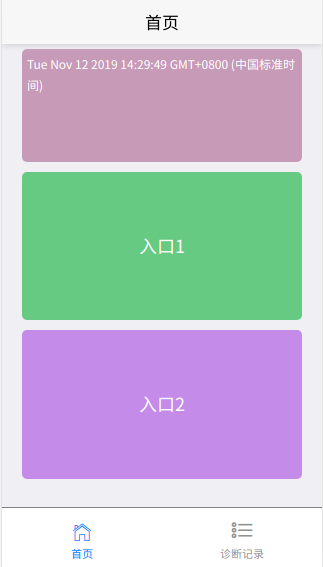
\includegraphics[width=3.5cm]{images/rukou.png}}
    \subfigure[新设计]{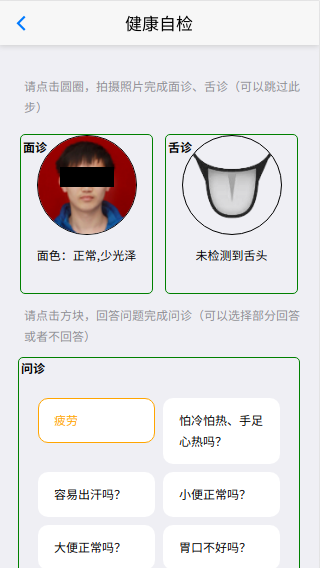
\includegraphics[width=3.5cm]{images/dialog1.png}}
    \subfigure[原设计]{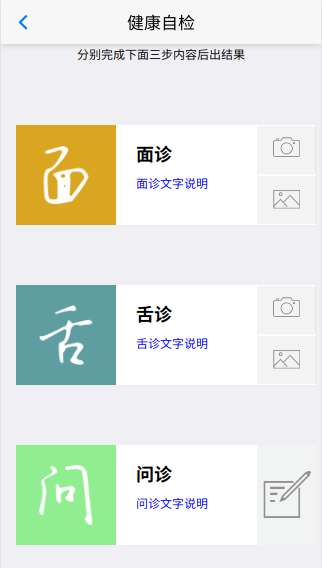
\includegraphics[width=3.5cm]{images/dialog2.png}}
    \caption{交互有效性实验}
    \label{fig:interface}
\end{figure}

我们在实验平台上,实现了一个用于对比的原型系统, 如图  \ref{fig:interface} 所示。在该原型系统的首页,有两个入口,新设计和原设计分别对应本文的设计和云中医的设计,两个设计的功能相同。

用户在进入实验原型系统的首页之后,可以自由选择通过哪一种入口,进入对应的界面完成诊断。

\subsection{原型系统实现}


\subsection{实验过程}

(1) 通过海报和社交媒体,招募到了10位对中医感兴趣的志愿者参与了本次实验。

(2) 在招募到志愿者之后,我们通过实验平台的问卷关联功能,让每个用户填写一个志愿者的基本信息的问卷,然后单独给每位志愿者介绍我们这次实验的背景和这次实验的整个流程。

(3) 之便让用户回家随意使用,我们则可以通过实验平台的日志管理功能观察用户的使用日志,实验期间用户也可以随时反馈使用感受。

(4)  在用户持续使用了大概两周之后,单独对每位用户进行深度访谈,通过录音的方式记录访谈数据。



\subsection{实验结果}


\begin{figure}[ht]
    \centering
    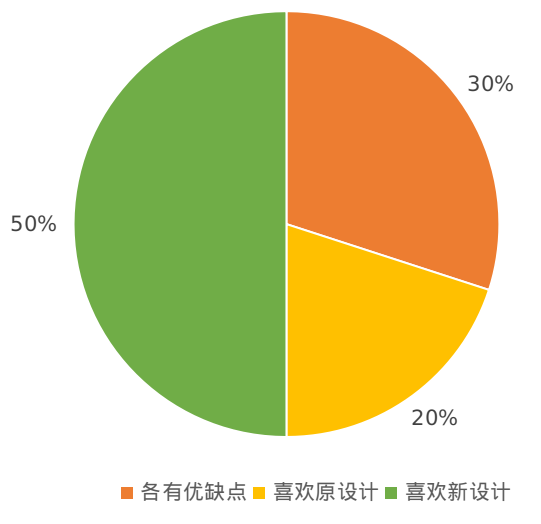
\includegraphics[height=8cm]{images/ui-exp.png}
    \caption{界面设计实验结果}
    \label{fig:ui-exp}
\end{figure}

如图 \cite{fig:ui-exp}所示, 有两位志愿者选择持续使用云中医的设计完成诊断, 五位用户更喜欢本文的新设计,而剩下三位用户觉得两种设计各有优缺点,具体原因如下:

\subsubsection{喜欢原设计}

原设计界面好看,问诊流程有完成感,并不想知道具体的症状对应什么细节。

原界面设计更符合常规,问诊是连贯的,首页内容很清楚。


\subsubsection{喜欢新设计}

新设计方便,单独做某一块检测;给的指示不空洞;有针对性和选择性。

新设计诊断透彻到位;可以选择性地做诊断,知道健康得分的构成,帮助了解中医知识,省时间。

新设计操作更简单,有选择性,但是问诊的选项太少,涵盖不全。

新设计界面丑,但原设计问卷很烦;新设计能实时显示舌诊结果。

设计挺好的,感觉更方便一些。


\subsubsection{各有优缺点}

界面设计更符合常规,问诊是连贯的,首页内容很清楚;新设计圆圈里的不同颜色有提示功能。

想按照顺序回答问卷,新设计问诊界面不舒服;但是新设计的选择性检测比较方便

新设计更方便,但一个一个问题点开很烦;原设计流程顺利,简单。

\subsubsection{总结}
通过实验,我们发现新的设计在一定程度上的确解决了本文在之前提到的可用性问题,但是也有部分年级较大的用户反馈新的设计过于复杂,没有依次做完面诊、舌诊、问诊的完成感。

\section{实验2:系统透明性验证}

已有大量的研究表明,增加系统的可解释性,是可以提高用户对系统的信任程度的。
考虑到诊断应用的特殊性,普通用户需要提高对应用的理解。因此我们在系统中加入算法的解释性,提升用户的体验。
而根据之前的用户调研的结果来看,由于当前诊断和打分模型存在改进的空间,部分的用户也对结果产生了怀疑或者对结果不理解。
在这个基础上,我们希望通过讲模型的诊断过程透明化,并对结果进行解释,来提高用户的交互体验。

\subsection{原型系统实现}

在具体代码实现的时候,系统对于是否过程透明、对结果进行解释是通过用户的类型来进行判断的。

对于每一个用户,我们通过哈希算法,对用户名计算哈希值,按照哈希值的奇偶性,将奇数用户归类为不透明用户,偶数用户归类为透明用户。
两类用户在进行面诊舌诊时的流程一样,但是透明用户能够看到背后特征提取算法和诊断算法的中间数据,同时系统为给出的诊断结果进行了解释。


解释在呈现的时候,大致可以分为两种:

(1) 结果中文字结果是有提示可以进行点击。如果用户点击了健康报告的分数,会通过弹窗进行详细的解释。

(2) 通过雷达图的方式直接显示对结果的影响,交互性比较强。

\subsubsection{面诊舌诊过程的解释}

\begin{figure}
    \centering
    \subfigure[不解释]{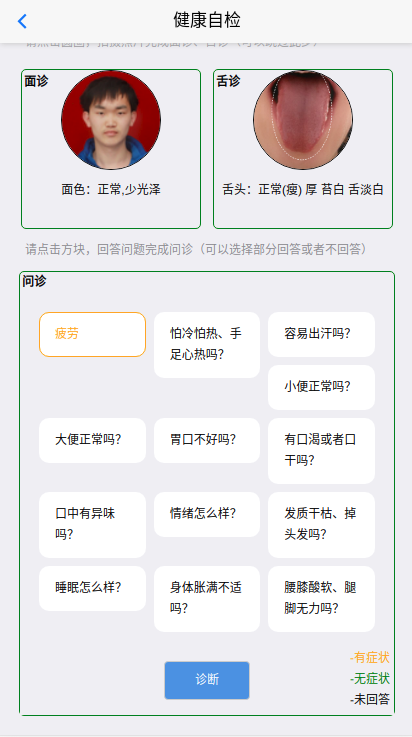
\includegraphics[width=3.5cm]{images/face_tongue.png}}
    \subfigure[解释]{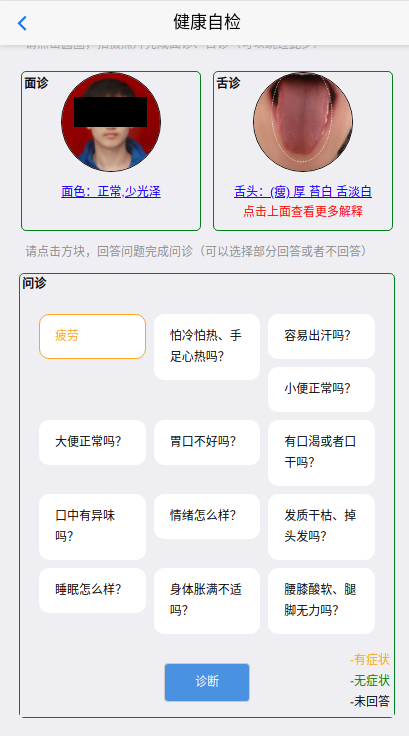
\includegraphics[width=3.5cm]{images/exp_face_tongue.png}}
    \subfigure[解释舌诊中间结果]{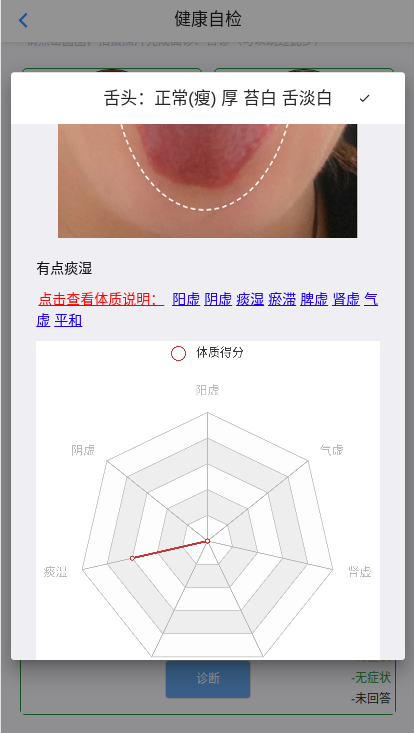
\includegraphics[width=3.5cm]{images/exp_tongue.png}}
    \caption{面诊舌诊的解释}
    \label{fig:face_diags}
\end{figure}

面诊和舌诊流程比较类似,添加解释主要体现在结果的解释,包括中间结果,和对各种体质倾向的影响。
这样用户查看解释之后,能够大致了解本次拍照是否成功,并且知道目前面诊的结果,会对最终的健康报告造成哪些影响。

如图 \ref{fig:face_diags} 所示:

(a) 普通用户只能看到结果。

(b) 透明类型的用户,可以通过点击结果,查看对结果的解释。

(c) 透明类型的用户,不仅可以看到当面诊断的中间结果,也能看到这次诊断的体质倾向得分。



\subsubsection{问诊的解释}

\begin{figure}
    \centering
    \subfigure[不解释]{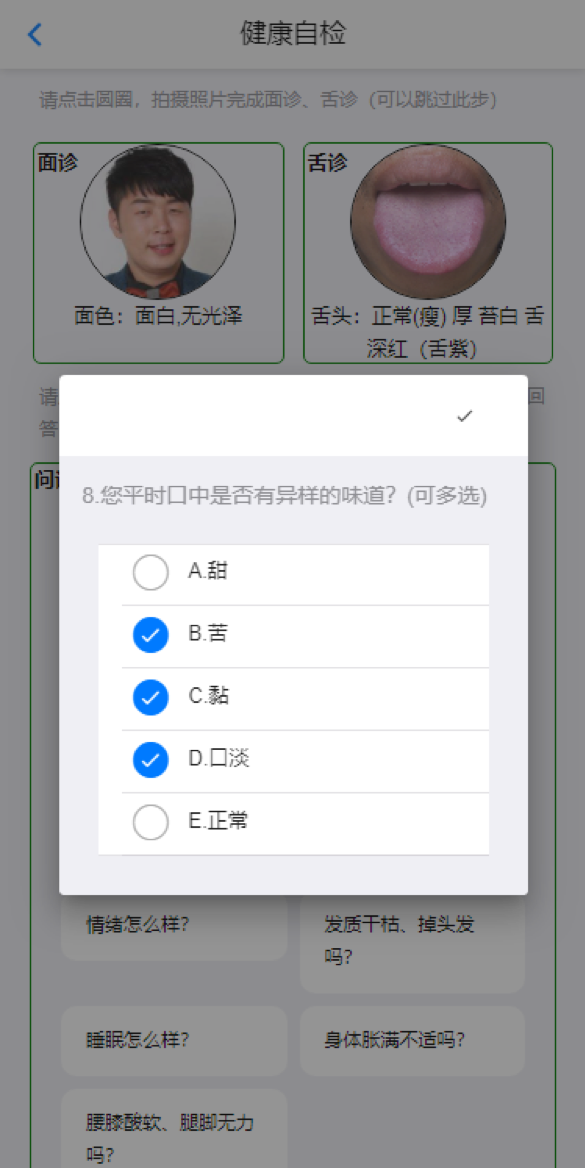
\includegraphics[height=10cm]{images/questions.png}}
    \subfigure[解释]{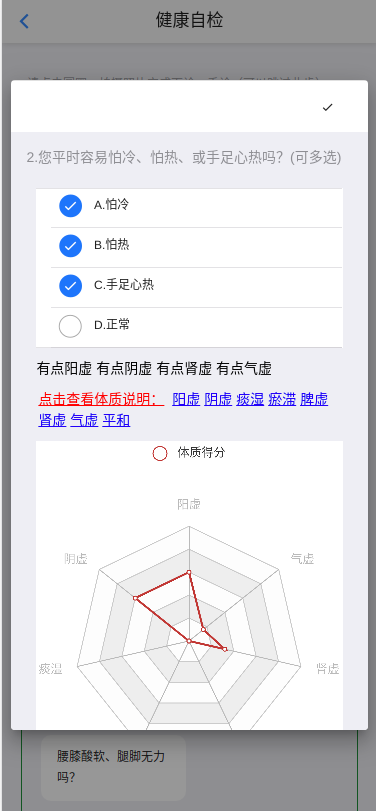
\includegraphics[height=10cm]{images/questions2.png}}
    \subfigure[解释体质术语]{
        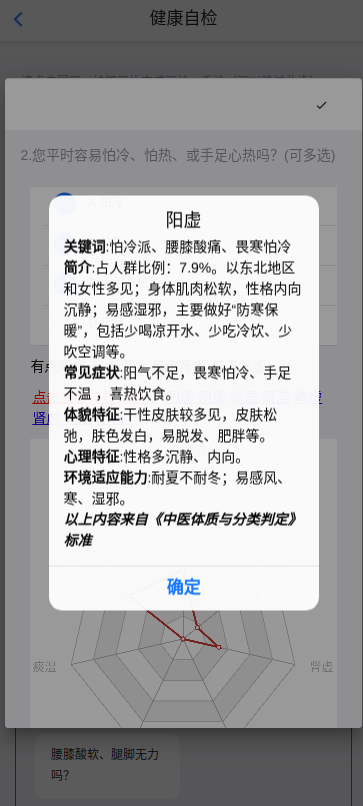
\includegraphics[height=10cm]{images/exp_phy.png}
    }
    \caption{问诊}
    \label{fig:questions}
\end{figure}

如图 \ref{fig:questions} 所示:

(a) 普通用户,回答问诊问题之后,没有任何提示或者解释。

(b) 透明类型的用户,在进行问诊过程中,可以立即看到每个答案对结果的印象,通过下方的雷达图显示了影响的体质倾向类型和具体的数值。
雷达图的更新是实时根据用户的选择进行更新的,提高了交互性。

(c) 对中医术语中,各种体质的解释,对于体质内容的解释文字引用自 《中医体质分类研究》标准。



\subsubsection{诊断结果的解释}
\begin{figure}[ht]
    \centering
    \subfigure[解释]{
        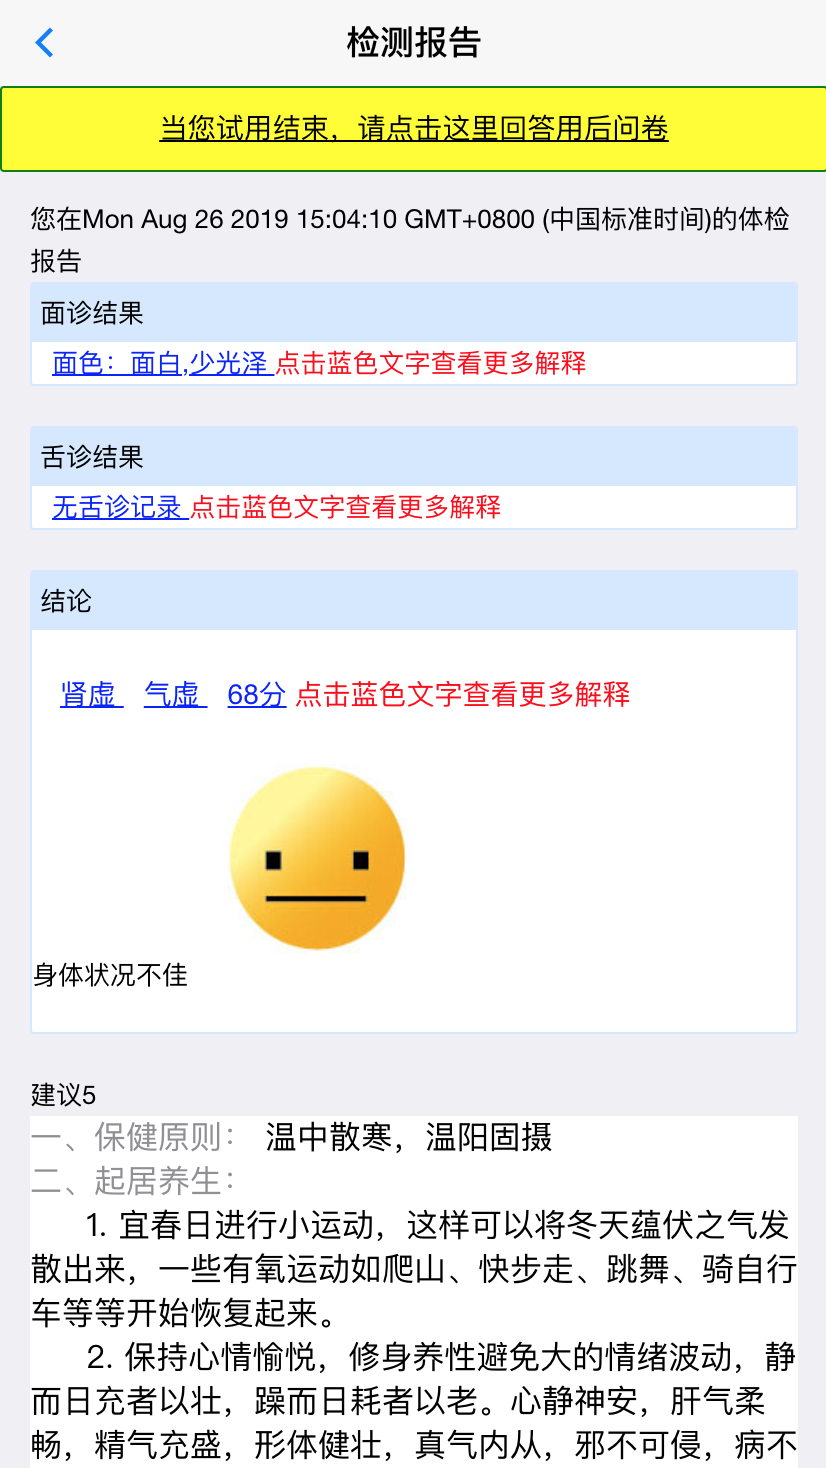
\includegraphics[height=10cm]{images/report3.png}
    }
    \subfigure[不解释]{
        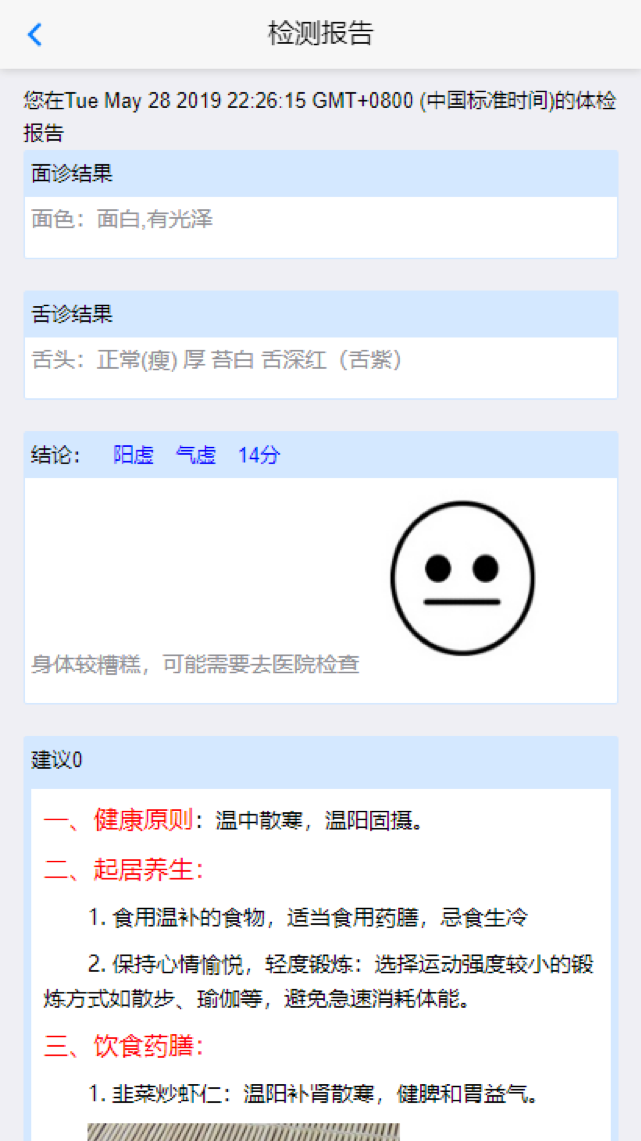
\includegraphics[height=10cm]{images/report.png}
    }
    \caption{诊断报告}
    \label{fig:my_label}
\end{figure}

普通用户在诊断结果页面,可以看到自己的健康分数和体质结果;透明用户可以点击诊断分数,了解这个分数是根据哪些指标,通过哪一个算法计算过来的。

可以点击查看的结果的解释有:面诊舌诊结果的解释,健康分数的解释,体质的解释。
 

\subsubsection{健康分数的解释}
问诊结果的解释主要是对用户透明诊断结果是如何计算出来的,以及那些问诊的问题对结果有影响,影响程度多少。

\begin{figure}[h]
    \centering
    \subfigure[相关问题]{
        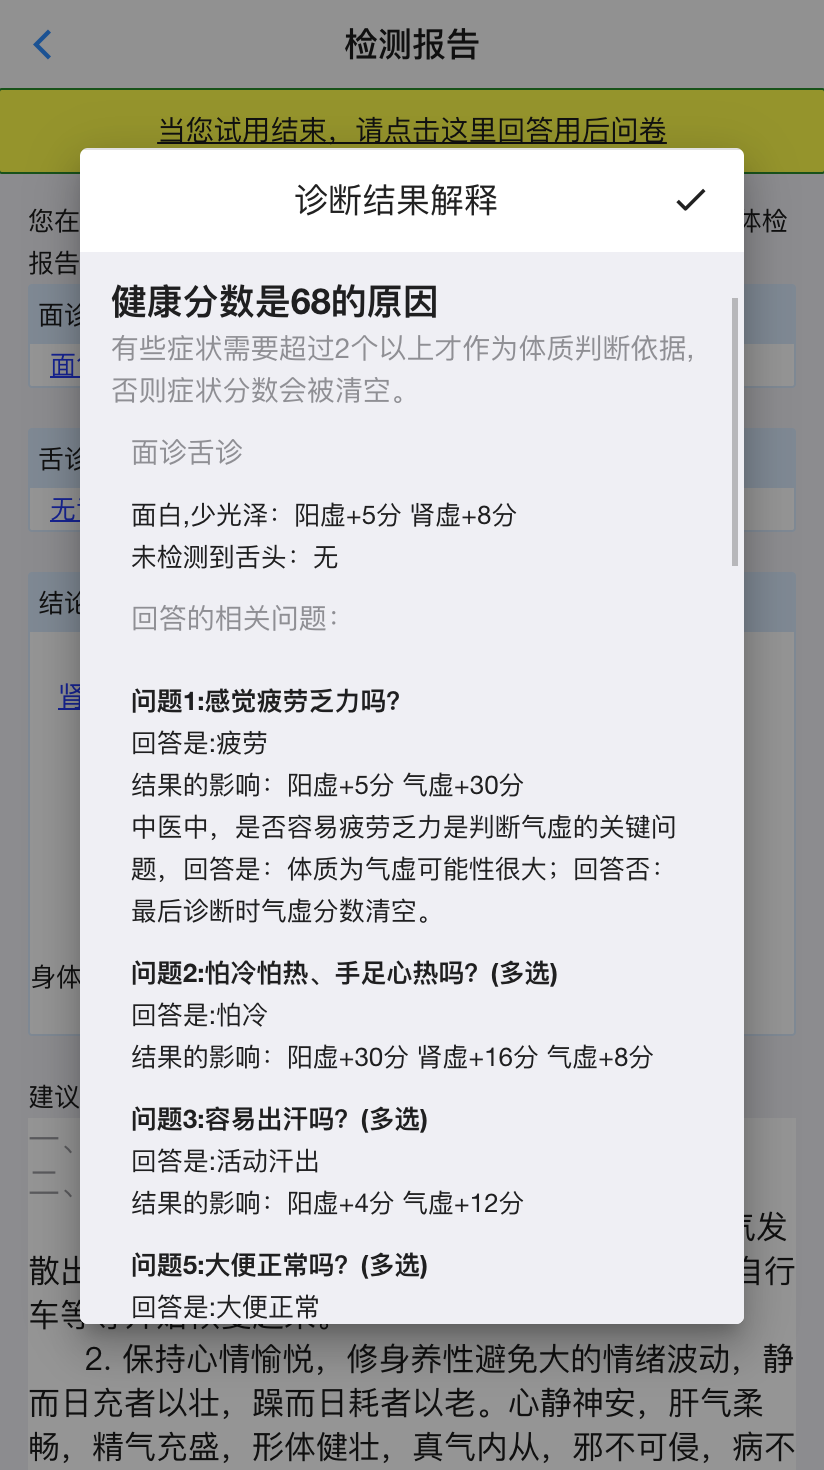
\includegraphics[height=7cm]{images/report7.png}
    }
    \subfigure[雷达图]{
        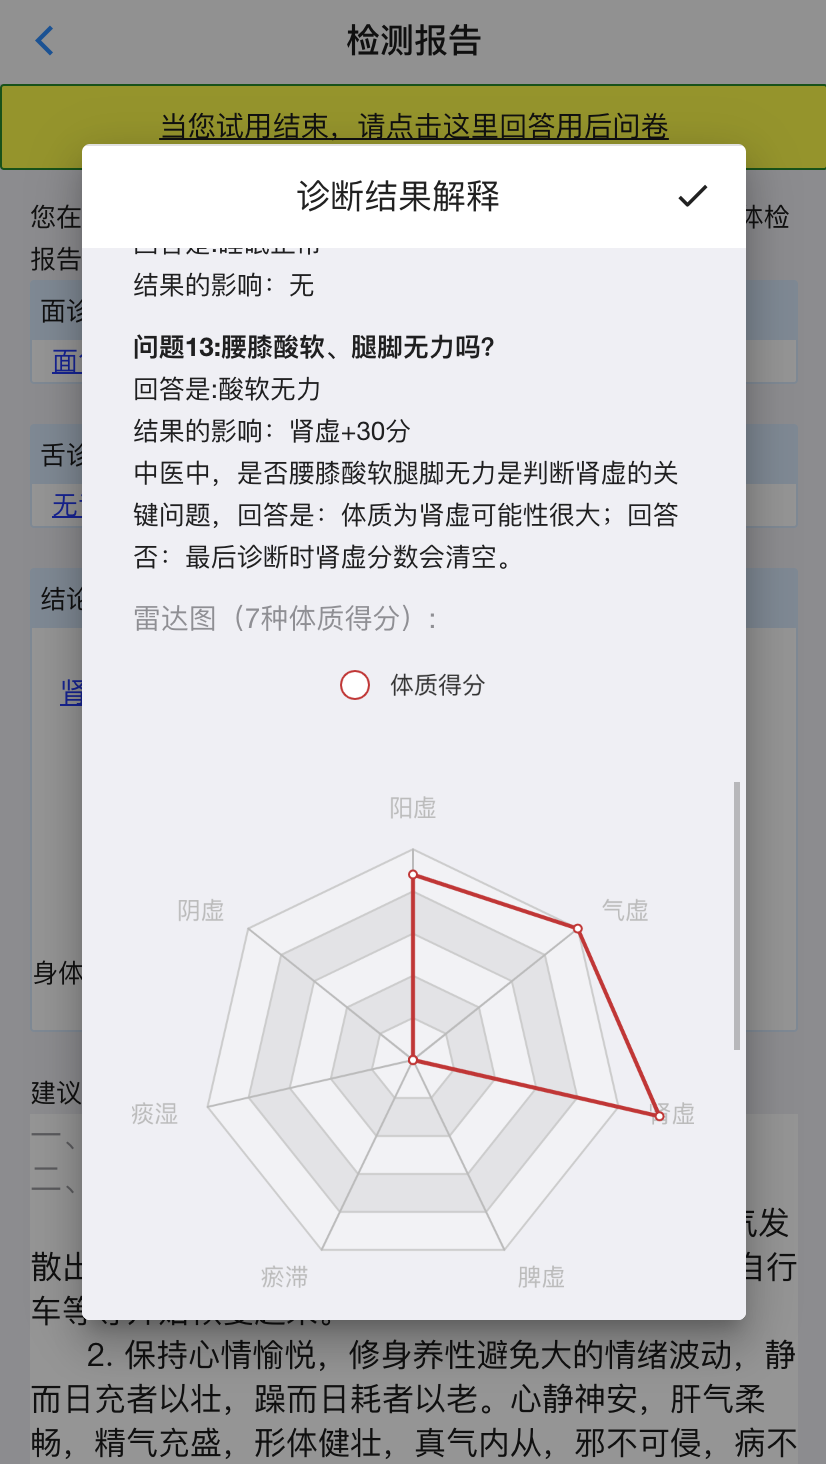
\includegraphics[height=7cm]{images/report8.png}
    }
    \subfigure[计算公式]{
        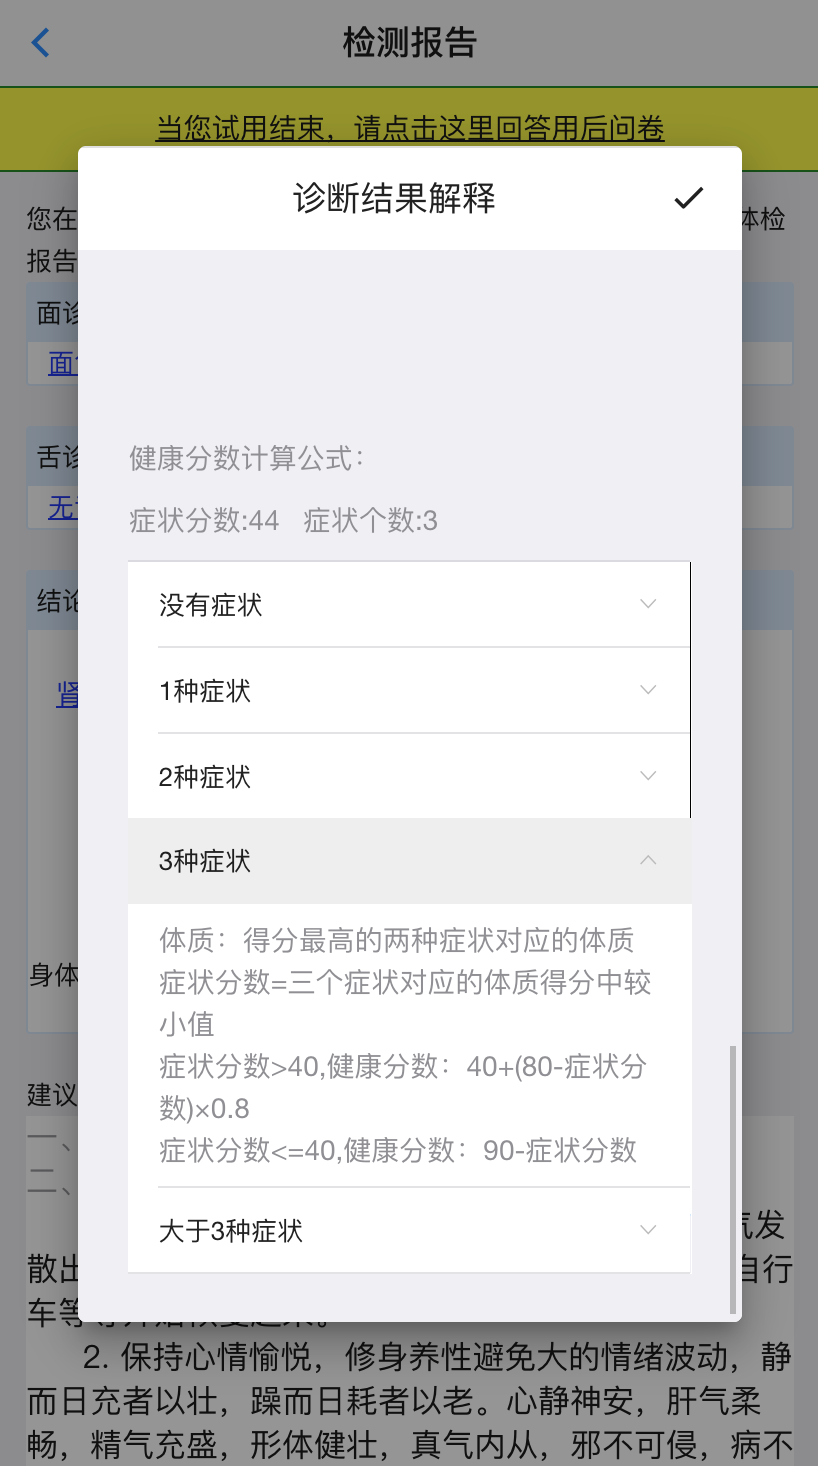
\includegraphics[height=7cm]{images/report9.png}
    }
    \caption{分数的解释}
    \label{fig:report_expalin_score}
\end{figure}

如图\ref{fig:report_expalin_score}所示,用户点击诊断页面的分数之后,弹窗里会显示分数相关的问题、雷达图和分数计算公式。

分数相关问题,展示了面诊舌诊对体质分数的影响和问诊对体质分数的影响,无影响的问题则不会显示。其中体质分数的变化分两种,一个是分数的累加,另一种是体质分数的清空。

雷达图对体质分数进行了汇总,给用户展示最终个人的体质倾向的结果。

根据诊断打分模型的内部算法,解释页面的计算公式一共有5种类别,我们使用选项卡的方式,将所有的打分计算公式全部透明给用户,并且默认打开当前计算公式的选项卡。

点击面诊结果,可以看到自己的面部舌部的对于整个诊断的影响。

点击体质分数,可以看到当次诊断中,面诊舌诊和用户自己回答的问题,哪些影响到了最后体质的判断。

\subsubsection{体质的解释}

\begin{figure}[ht]
    \centering
    \subfigure[面诊的解释]{
        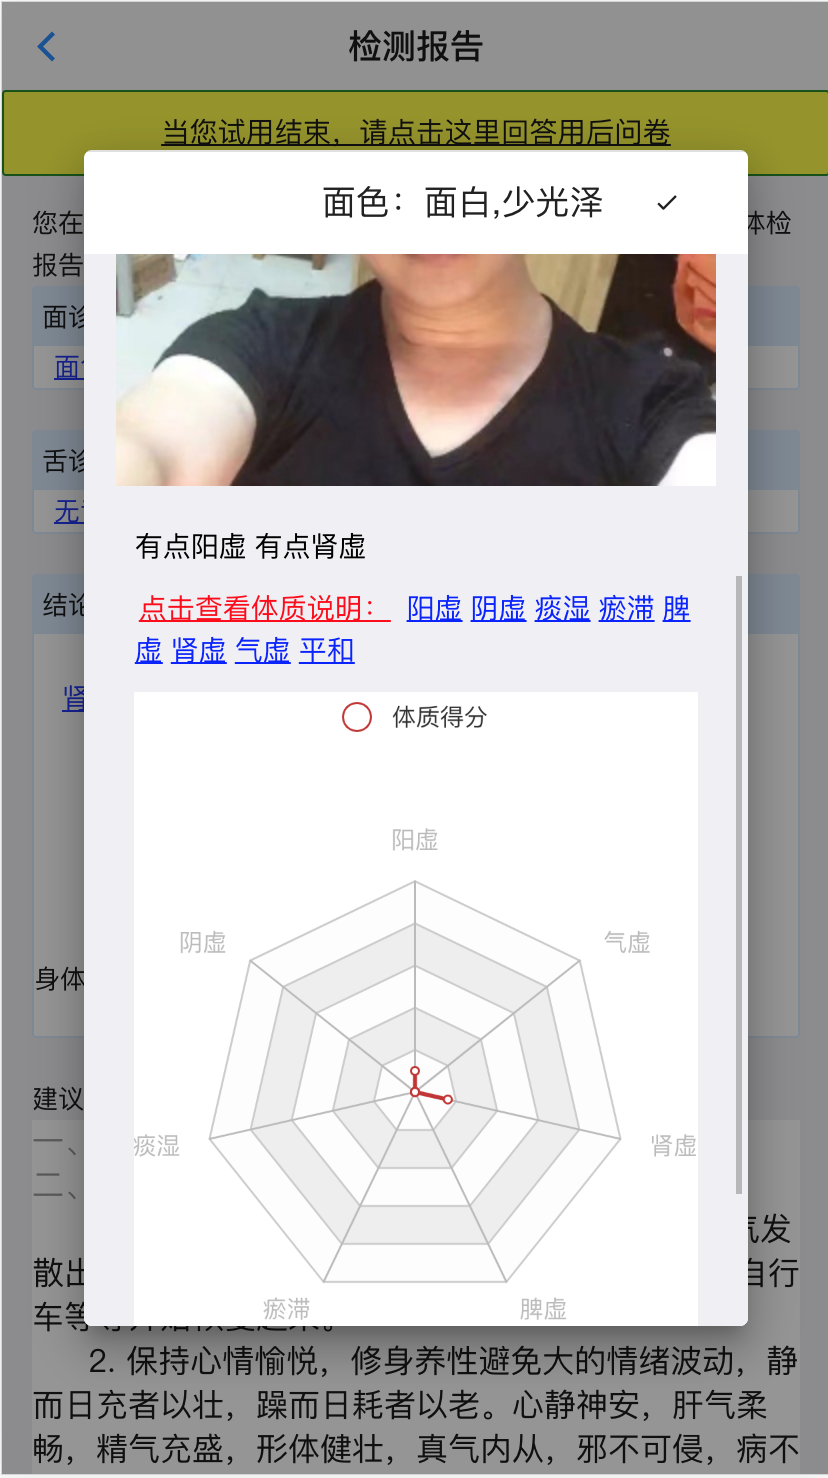
\includegraphics[height=7cm]{images/report4.png}
    }
    \subfigure[概念的解释]{
        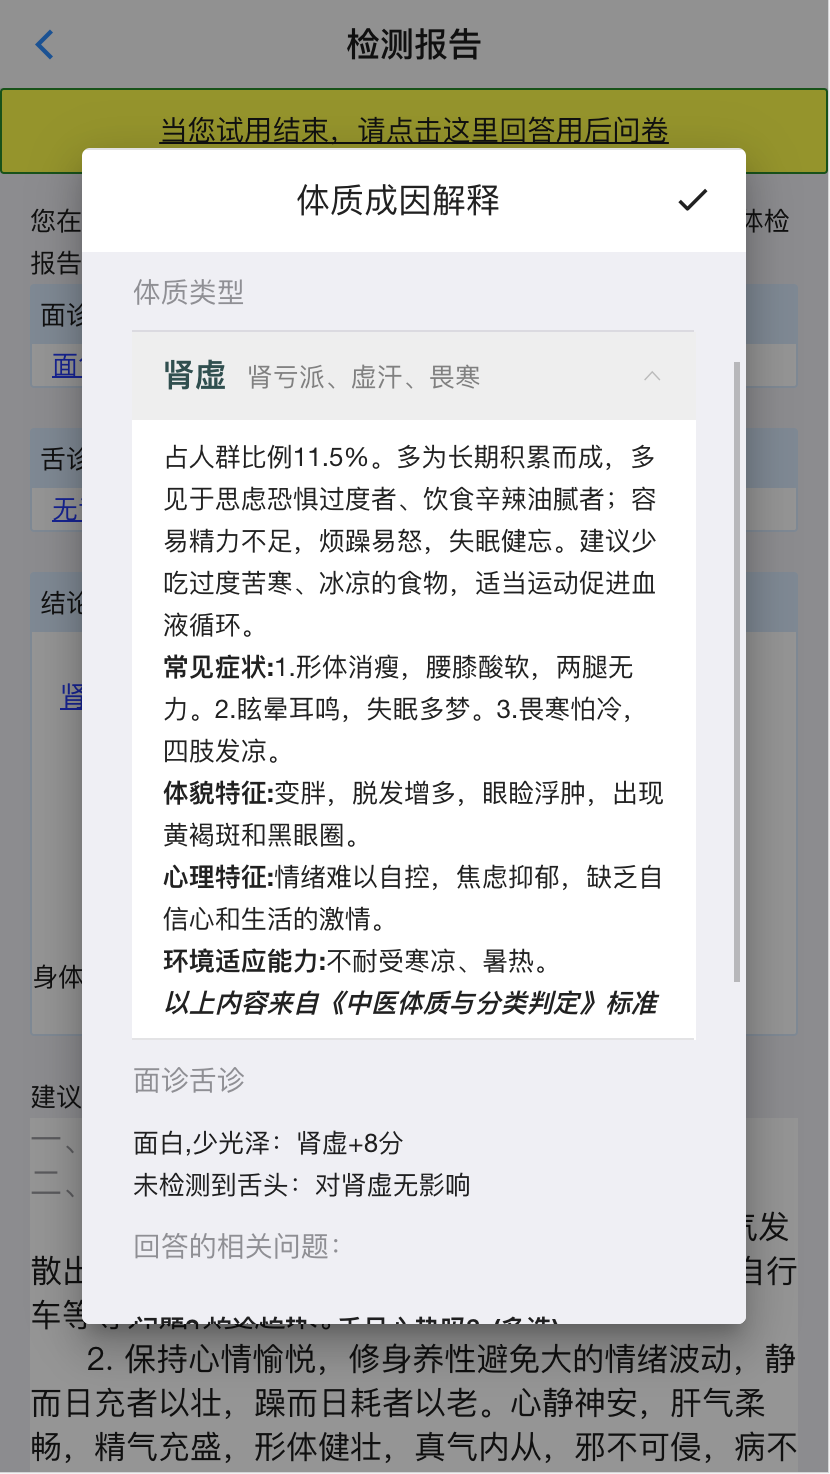
\includegraphics[height=7cm]{images/report5.png}
    }
    \subfigure[体质相关问题]{
        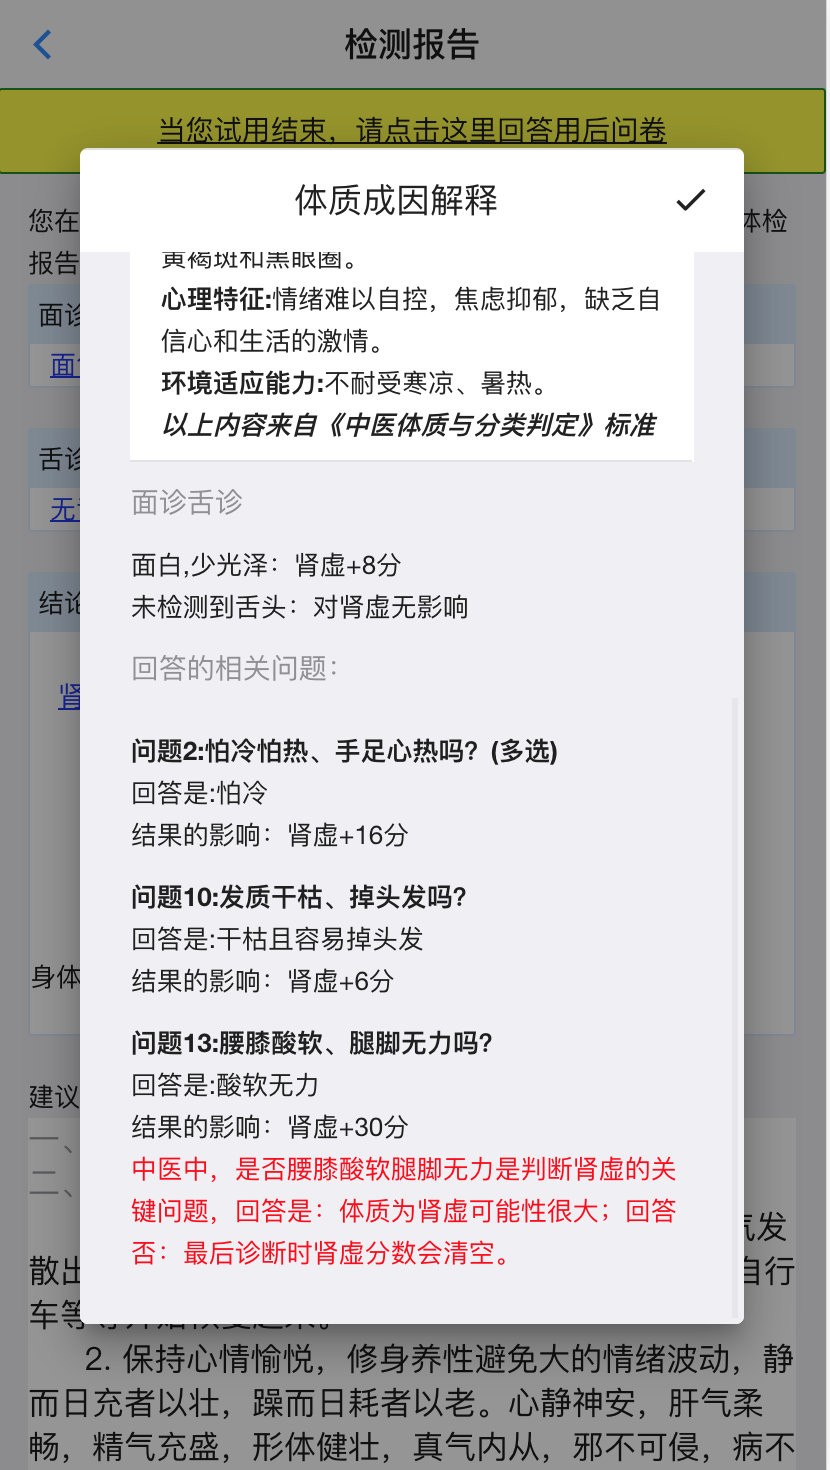
\includegraphics[height=7cm]{images/report6.png}
    }
    \caption{诊断结果的解释}
    \label{fig:report_explain_phy_1}
\end{figure}


% \section{反馈调研}
% 在新系统完成之后,我们采访了16名用户。
% 在本次调研过程中,用户试用的是同时有新旧界面的版本,除了第一次介绍使用的时候,我们会让用户两个版本都是使用一下,后续不做限时。用户具体使用的时候可以根据自己的喜好选择。
% 经过回访,新设计的界面达到了预期,大部分用户觉得使用起来更加地方便。
% 不过值得注意的是,也有少部分的用户喜欢原设计的将面诊,舌诊,问诊分开为三步进行的方式,因为这样比较符合日常生活的习惯。


\subsection{实验设计}
我们通过在各大社交平台发布海报招募,如图\ref{fig:poster},以及使用问卷星的样本服务, 经过筛选之后,一共招募了100位左右的用户。
\begin{figure}[ht]
    \centering
    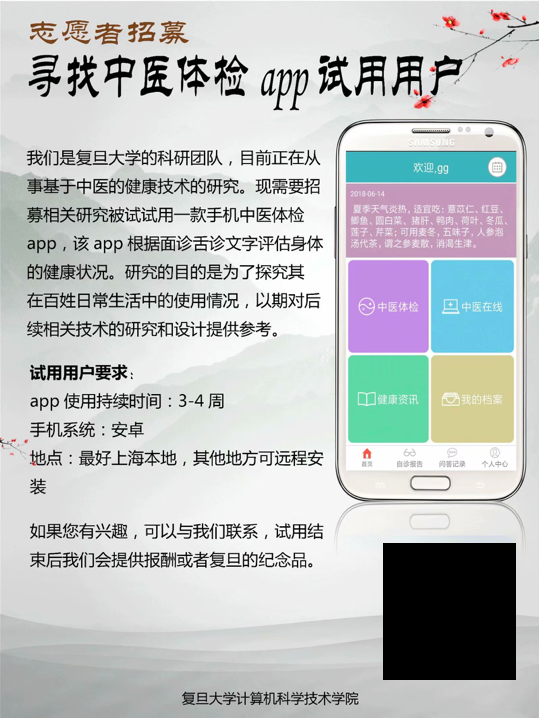
\includegraphics[height=8cm]{images/poster.png}
    \caption{招募海报}
    \label{fig:poster}
\end{figure}
\section{实验流程}

每个用户的实验流程如下:

(1)用户通过扫描二维码,或者通过我们给定的链接,进入问卷星调查问卷。

(2) 完成调查问卷之后,自动进入云中医在线app。通过调用问卷星提供的企业用户接口, 同时把问卷星的问卷id通过ssojump传给云中医在线应用。通过ssojump中的问卷id, 完成自动登陆, 登陆的用户id为wjx-{问卷星id}, 透明类别为通过问卷星id哈希得到。

(3) 在用户完成一次面诊之后,会在健康诊断页面下,看到一个跳转链接,可以选择填写用后问卷。

这样就把调查问卷信息,云中医应用使用日志和用后问卷数据关联起来了。


\section{实验数据获取}
每个用户在参与实验之后,我们可以得到调查问卷的数据,云中医的使用日志,已经用后问卷的数据。

调查问卷: 序号,提交答卷时间,所用时间,来源,来源详情,IP,个人信息	我相信中医养生,了解中医养生,平时注重养生,经常去看中医,希望自己的生活方式更健康,对学习相关中医养生知识感兴趣,认为中医面诊可以了解健康情况,认为中医舌诊可以了解健康情况,认为智能系统可以自动评估健康情况,随机顺序的中医知识问题

用后问卷: 序号,提交答卷时间,所用时间,来源,来源详情,IP,云中医的诊断结果,结果的信任程度,对结果的理解程度,是否愿意使用类似应用,随机顺序的中医知识问题

用户使用日志: 序号,用户名,设备信息,操作名,操作信息,日期 

个人信息包括性别,年龄段,受教育水平,职业,城市,健康状态等。

\subsubsection{关联规则}
对于同一个用户在一次实验过程中,若调查问卷的序号为ID, 则此次用户使用日志的用户名为wjx-ID, 用户问卷的来源详情为wjx-ID。 
通过这个对应关系,我们就可以利用实验平台提供的问卷关联的功能,把三个表的信息,合并到一个表中,通过django-admin导出下载,最终得到特征如表\ref{tab:exp_data}所示。


\begin{table}[h]
    \centering
    \begin{tabular}{ll}
        \toprule
        字段 & 描述 \\ 
        \midrule
        序号 & 调查问卷序号 \\
        性别 & 男/女/未知 \\
        教育程度 & 本科以下/本科/本科以上 \\
        工作类型 & 计算机相关/计算机不相关 \\
        用户类型 & 透明/不透明 \\
        健康得分 & 云中医应用给出的分数 0-100 \\
        信任 & 对结果的信任程度 1-5 \\
        理解 & 对结果的理解程度 1-5 \\
        前健康知识得分 & 使用云中医之前的健康知识得分 \\
        后健康知识得分 & 使用云中医之后的健康知识得分 \\
        查看了哪些解释 & 使用过程中查看的解释类型 \\
        \bottomrule
    \end{tabular}
    \caption{实验数据汇总}
    \label{tab:exp_data}
\end{table}

表格 \ref{tab:exp_data}的字段说明如下:

工作类型: 根据调查问卷的数据,用户自由填写的职业类型有很多,为了便于分析,我们把 IT经理,IT软件设计, hr, it, 互联网, 技术研发, 技术研发人员, 技术经理, 电脑工程师, 研发, 科研, 程序员, 计算机, 软件工程师, 软件开发工程师, 通信, 通讯等归为it相关。

信任、理解: 这两个字段来自用后问卷调查表,取值范围为1-5的整数。

健康知识得分: 使用云中医应用前后的健康知识得分,使用的是用户回答正确中医知识的个数。

用户类型:透明类型的用户才能看到对结果以及术语的解释。

查看了哪些解释: 通过检索日志中关键字获取,包括面诊过程,舌诊过程,体质术语介绍,诊断报告的:面诊结果,舌诊结果,健康分数,体质,分数计算公式等。

\subsection{实验结果}



% 同时实验分析,我们可以得出,增加解释可以提高用户对应中医知识的理解。

% 和看解释有关, 用 二元逻辑回归

% 把用户进行筛选,看了解释和没有看解释的

% 有解释的,看了没没看的(为什么看了,为什么没看), 

% 相关性分析,用于分析自变量

% 挑选相关性比较低的,放到后续的模型中 , 不加*,是很弱的 0.4-0.6比较强

% 了解中医养生,平时注重养生,了解中医养生
% 相信中医,了解中医

% 有没有看解释和it相关性不高

% 看了解释的影响:
% 独立样本t检验,差异性分析,没有显著差异

% 找最相似的不看解释的用户和看了解释的用户对比: 
% 对结果的信任和理解程度,两个样本没有显著差异



% 量化结果

% 定性实验

\subsection{附加实验:结构性访谈}

定量的数据分析,由于用户的参与度不是很高、问卷设计过于复杂等原因,我们无法得出哪些因变量如对结果的信任与是否有解释的相关性,于是我们在该次实验之后,对实验的参与者附加了一个深度访谈。

本次实验,我们同样实现了一个原型系统,界面和流程与上一个实验完全相同,但是去掉了用户登录时的随机分配用户角色,而是添加了一个开关。
当开关关闭的时候,系统不会对结果进行解释;当开关打开的时候,系统会对诊断过程和诊断结果进行详细的解释。

在使用过程中,我们首先让用户试用有解释或者没有解释的版本,让用户随时讨论自己内心的想法。然后我们切换开关,让用户再一次使用。最后对用户进行一次深度访谈。

通过定性访谈,我们发现日常面诊环境下,可解释性有以下结论:

\subsubsection{添加解释能够提高用户对诊断结果的接受程度}

(1)用户知道背后的原理之后,如果结果不符合自己的预期,会尝试从自己方面的原因解释为什么不是这个结果,是不是操作不规范。

(2) 知道深度学习需要大量的数据,目前数据量可能不足,有一定的错误率是正常的。

\subsubsection{添加解释能够增加对系统的信赖程度}

(1) 用到了实际的深度学习的技术, 觉得更加可信赖

(2) 觉得研发的机构比较权威,系统比较可靠

但是在对结果的解释时,没有提到体质判决的依据

\subsubsection{本文使用的添加解释的方法对于提高中医的理解,帮助不大}
(1)用户没有兴趣需要更加复杂的机制吸引用户深入学习。

(2) 术语太多,不好理解

(3) 时间太短,学习效果一般

\subsubsection{添加解释的解释方法,需要更加灵活有趣的方式,而不只是图表的形式}
(1)通过讲故事的形式,图文并茂,配上视频

(2) 通过系统中测试数据,通过和健康的对比的方式

当前缺点: 内容太多,太复杂, 只需要解释关键部分,判决依据就可以了

\subsubsection{简单的解释可能可能会让用户忽略}
(1) 文字提示的形式不明显,不知道可以点击(可以做成消息提醒的小红点的形式)

(2) 看到解释的提示,但是自己对结果没有疑惑

(3) 想尽快完成本地诊断的流程


\section{本章小结}


